\documentclass{article}
\usepackage{graphicx}
\graphicspath{./}

\title{Trabalho parcial 02: diagrama de atividades}
\author{Gustavo Guerreiro, João Martinho}
\date{1º de outubro de 2025}

\setlength{\oddsidemargin}{-0.5cm}
\setlength{\evensidemargin}{-0.5cm}
\setlength{\textwidth}{17cm}
\setlength{\topmargin}{-1.5cm}
\setlength{\textheight}{24cm}

\begin{document}

\maketitle

\section{Resumo}

O nosso trabalho usa técnicas clássicas de pré-processamento e segmentação para distinguir e contar os núcleos celulares dos neutrófilos da base de imagens fornecida. A \textit{pipeline} do processamento começa com técnicas mais simples de segmentação e avança para ténicas mais robustas, passando pela análise de cor, intensidade e bordas, e finaliza com o uso do algoritmo Watershed.

\section{Tabelas}

Abaixo estão duas tabelas mostrando a quantidade de núcleos encontradas pela nossa solução em cada imagem. A primeira tabela mostra os resultados obtidos com os linfócitos (3 imagems), e a segunda, com os neutrófilos (10 imagens).

\begin{table}[h]
\centering
\begin{minipage}{0.45\textwidth}
\centering
\begin{tabular}{|c|c|}
\hline
\multicolumn{2}{|c|}{Linfócitos} \\
\hline
linfocito00.png & 3 \\
linfocito01.png & 2 \\
linfocito02.png & 4 \\
\hline
\end{tabular}
\end{minipage}
\hfill
\begin{minipage}{0.45\textwidth}
\centering
\begin{tabular}{|c|c|}
\hline
\multicolumn{2}{|c|}{Neutrófilos} \\
\hline
neutrofilo00.png & 4 \\
neutrofilo01.png & 3 \\
neutrofilo02.png & 2 \\
neutrofilo03.png & 4 \\
neutrofilo04.png & 3 \\
neutrofilo05.png & 2 \\
neutrofilo06.png & 4 \\
neutrofilo07.png & 3 \\
neutrofilo08.png & 2 \\
neutrofilo09.png & 4 \\
\hline
\end{tabular}
\end{minipage}
\end{table}

\section{A \textit{pipeline}}

\subsection{Preparação do ambiente}

Inicialmente, importamos as bibliotecas necessárias, nomeadamento o OpenCV, o NumPy e o Matplotlib, responsáveis, respectivamente, pelas operações de visão computacional, manipulação numérica e visualização gráfica.

\subsection{Isolamento de células}

A função de isolar célula converte a imagem para escala de cinza e aplica um theshold binário para separar a célula do seu fundo escuro, substituindo-o por branco a mantendo apenas a região da célula, que por sua vez é retornada ao espaço de cores RGB.

\subsection{Segmentação simples por intensidade}

O notebook executa um laço que percorre as dez imagens de neutrófilos, convertendo cada uma para tons de cinza e aplicando threshold para binarizá-las. Os resultados são exibidos; neles, observa-se que a segmentação baseada em intensidade separa parcialmente os elementos de interesse.

\subsection{Ajustes interativos de cor}

A seguir, o notebook aplica um recurso com barres deslizantes (trackbars) no OpenCV. Essas barras permitem ao usuário/programador ajustar dinamicamente os limites de matiz, saturação e valor no espaço HSV, e observar o efeito da máscara sobre as imagens do dataset. Esta fase serve para calibrar intervalos de cor capazes de destacar os núcleos celulares.

\subsection{Segmentação sistemática de núcleos}

Definidos os limites, a função de segmentar e mostrar núcleo aplica os parâmetros fixos a uma imagem. Nesta etapa, são exibidas lado a lado a fotografia original, a máscara em tons de cinza e a região do núcleo segmentada.

\subsection{Mapas de probabbilidade}

A função de criar mapas de probabilidade do núcleo avalia a chance de cada pixel pertencer ao núcleo com base em três fatores: a faixa de matriz, a saturação (normalmente mais alta nos núcleos) e a intensidade luminosa. Para dar maior peso aos valores centrais da faixa de cor, utilizamos uma função gaussiana. O resultado é normalizado e binarizado automaticamente pelo método de Otsu.

\subsection{Refinamento com bordas}

A função decriar mapa de probabailidade preciso incorpora gradientes de borda calculados pelo operador de Sobel. O mapa final é obtido ao multplicar-se a probabilidade de cor pela ``anti-borda'', isto é, uma medida que valoriza áreas internas e atenua regiões de contorno, o que aumenta a precisão, reduz falsos positivos e destaca apenas as áreas centrais dos núcleos.

\subsection{Segmentação com Watershed}

O algoritmo Watershed aplica limiares e operaões morfológicas para obter uma máscara limpa. Em seguida, usa a transformada de distância para identificar com mais confiança os centros dos núcleos, distinguindo, das áreas de primeiro plano, o fundo e as regiões de incerteza. O resultado final é uma segmentação precisa e seus contornos são desenhados em vermelho sobre a imagem original.

\subsection{Processamento em lote}

Por fim, o notebook organiza esse fluxo em um processo em lote e aplica a versão final da segmentação a todas as imagens de neutrófilos da pasta. O usuário pode então visualizar cada resultado com os núcleos devidamente segmentados.

\section{Diagrama de atividades}

Na próxima página está o diagrama de atividades (no estilo flowchart) que representa a nossa solução do trabalho, renderizado pela ferramenta Mermaid.

\begin{figure}[h!]
    \centering
    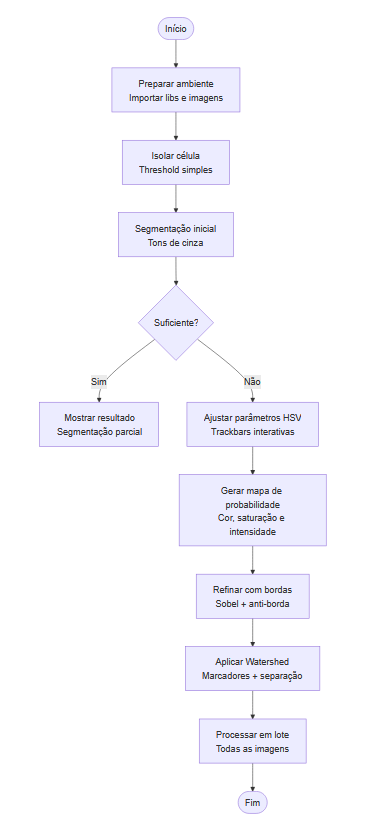
\includegraphics[width=0.6\textwidth]{diagrama.png}
    \caption{O diagrama de atividades}
    \label{fig:exemplo}
\end{figure}


\end{document}
